\subsection{Entity-Relationship Schema}

\begin{center}
	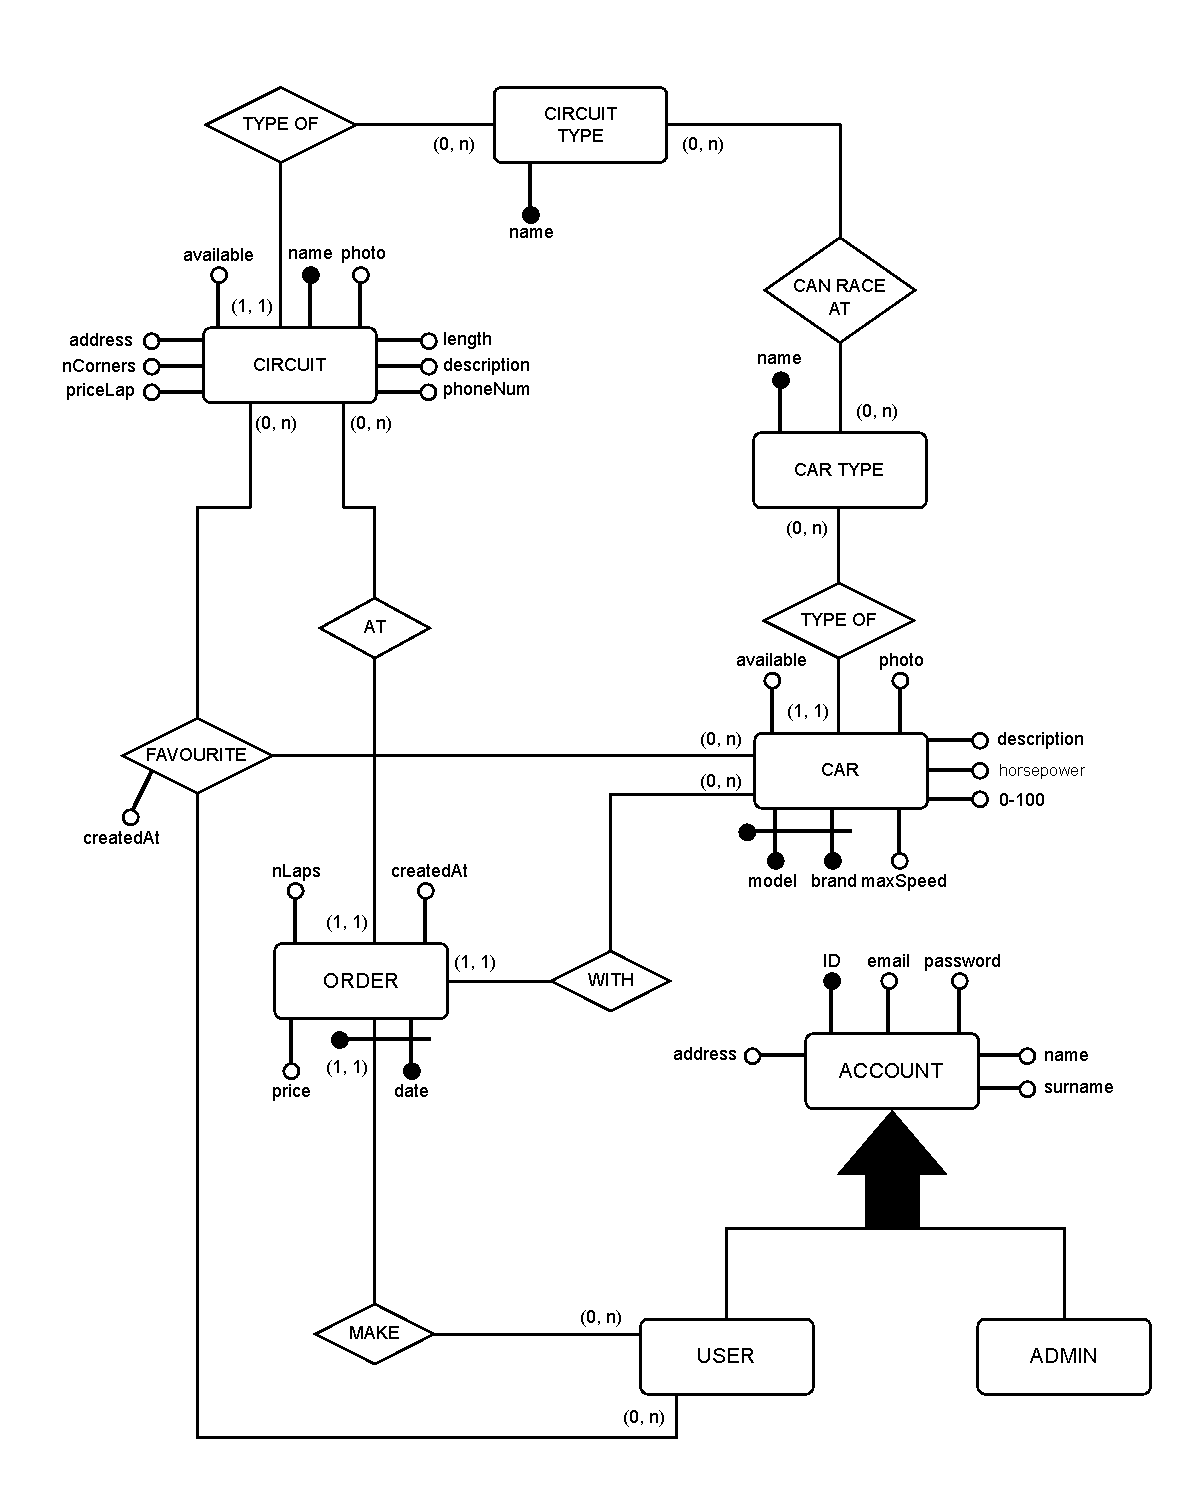
\includegraphics[scale=0.55]{ERSchema.pdf}
	\captionof{figure}{ER schema of WACAR}
	\label{ERSchema}
\end{center}

The ER schema contains the following entities:
\begin{itemize}
	\item \textbf{account}:the account contains both the account for the users of the web app and the admin that manages the contents of the tables. It has an email (type TEXT) and a password (type TEXT) that it uses for signing in. Then, it has the name (type CHARACTER VARYING), the surname (type CHARACTER VARYING) and the address (type TEXT). Finally, it has the attribute type that is an enumerator and it can assume value "USER" or "ADMIN" which specifies the type of the account. An account have a 0-N relationship with entity \textit{order}, so that it can make more than one order. Finally, an account can also add a pair \textit{car-circuit} in a bookmarks list represented by the relationship \textit{favourite}.
	\item \textbf{car}: it represents the entity for the car users car drive. Its primary key is composed by the brand and the model of a car (both type CHARACTER VARYING), some data are about the performance of the car such as the horsepower (type INTEGER), the 0-100 acceleration (type NUMERIC) and the maxSpeed (type INTEGER). For more general information there is the description (type TEXT). Finally, it has a foreign key for the type of the car (e.g. 'supercar'), an image (type BYTEA) and an attribute available (type BOOLEAN) that defines if the car is available for new orders.
	\item \textbf{circuit}: this entity represents the circuit in which a user can race. It is identified by its name (type CHARACTER VARYING). Then, it contains the address (type TEXT), the price for doing a lap (type INTEGER) and some characteristics such as the length (type  INTEGER), the number of corners (type INTEGER) and a general description (type TEXT) with also an image (type BYTEA). Finally, it has a foreign key for the type of circuit (e.g 'tarmac') and, as in car entity, it has the attribute available (type BOOLEAN). 
	\item \textbf{circuitType} and \textbf{carType}: the first entity contains the name (type CHARACTER VARYING) of the type of a circuit, while the second entity contains the name (type CHARACTER VARYING) of the type of a car. Those entities are related to each other by the 0-N \textit{can race at} relationship. This relationship saves the suitability between a type of circuit and a type of car: for example, if a pair circuitType-carType is composed by 'tarmac'-'supercar', then this means that a supercar can race on all the circuits of that type. Otherwise, if for example the pair 'rallycross'-'supercar' is not present, then the supercar cannot race on this type of circuit.
	\item \textbf{order}: its primary key is an id (type INTEGER). It contains the email of the \textit{account} that has made the order and the date (type DATE) in which the user will have the experience. It also contains lapsNumber (type INTEGER), that is the number of laps for this booked session, and the price (type INTEGER) of the order. Then, to specify in which circuit and with which car the user wants to prenote, the order has the reference to the entity \textit{circuit} and to the entity \textit{car}.
\end{itemize}
